\chapter{Resultados e Validação Prática}
\label{cap:resultados}

A aplicação foi submetida aos testes propostos para validar as propriedades fundamentais do esquema FullIdent em um cenário prático. O desenvolvimento de uma interface gráfica interativa (Dear ImGui) permitiu que as etapas matemáticas de extração de chaves e roteamento de e-mails pudessem ser operadas visualmente. A seguir, são demonstrados os fluxos de funcionamento do sistema.

\section{Registro e Autoridade de Chaves (PKG)}

Diferente da infraestrutura de chaves públicas (PKI) tradicional baseada em certificados, no esquema IBE a chave privada deve ser gerada por uma autoridade central confiável (PKG -- \textit{Private Key Generator}).

A Figura \ref{fig:registro} ilustra a tela inicial do \textit{IBE Mail}, onde o usuário solicita o registro de uma identidade arbitrária (por exemplo, um e-mail).

\begin{figure}[htb]
    \centering
    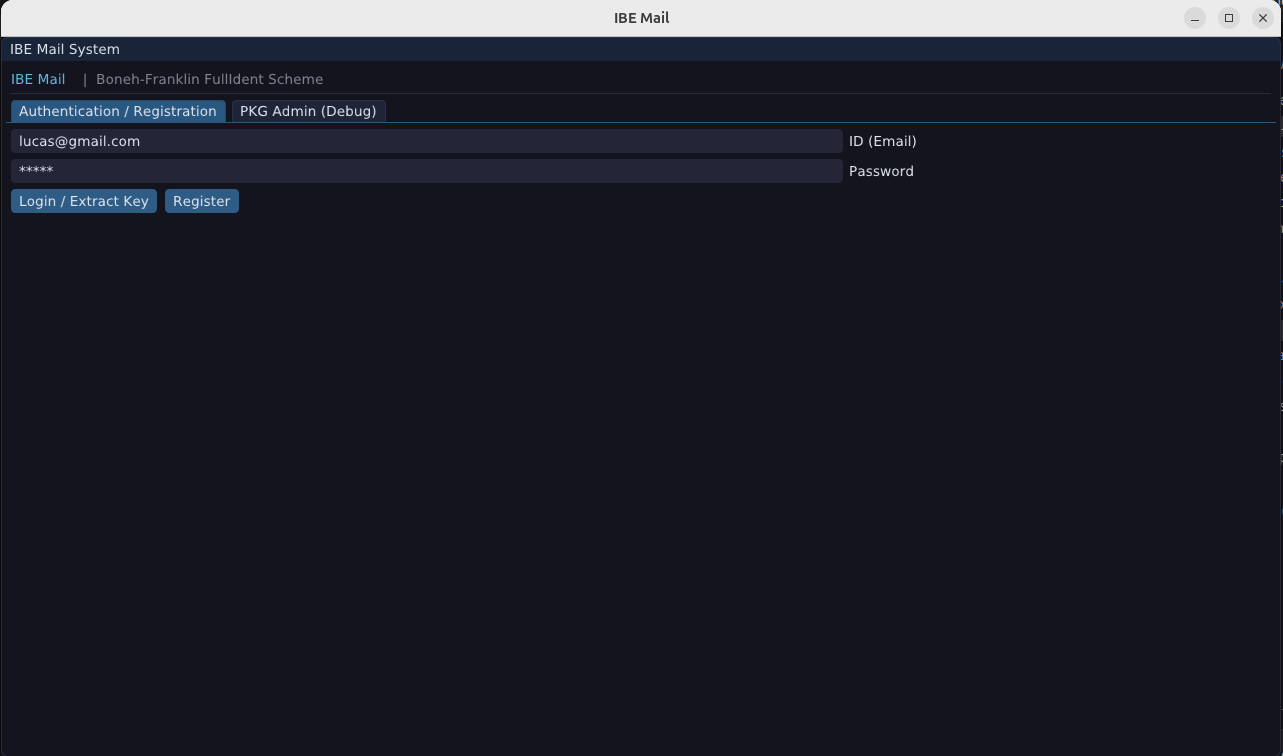
\includegraphics[width=0.9\textwidth]{images/1_registro.png}
    \caption{Tela de autenticação e solicitação de registro de identidade.}
    \label{fig:registro}
\end{figure}

Após o registro, a solicitação fica pendente no painel do administrador (Figura \ref{fig:pkg_pending}). O administrador do PKG, detentor do segredo mestre (\textit{Master Secret}), é responsável por aprovar a identidade do usuário. Ao clicar em \textit{Approve} (Figura \ref{fig:pkg_approved}), a chave privada do usuário é matematicamente derivada sobre a curva elíptica supersingular e armazenada em disco.

\begin{figure}[htb]
    \centering
    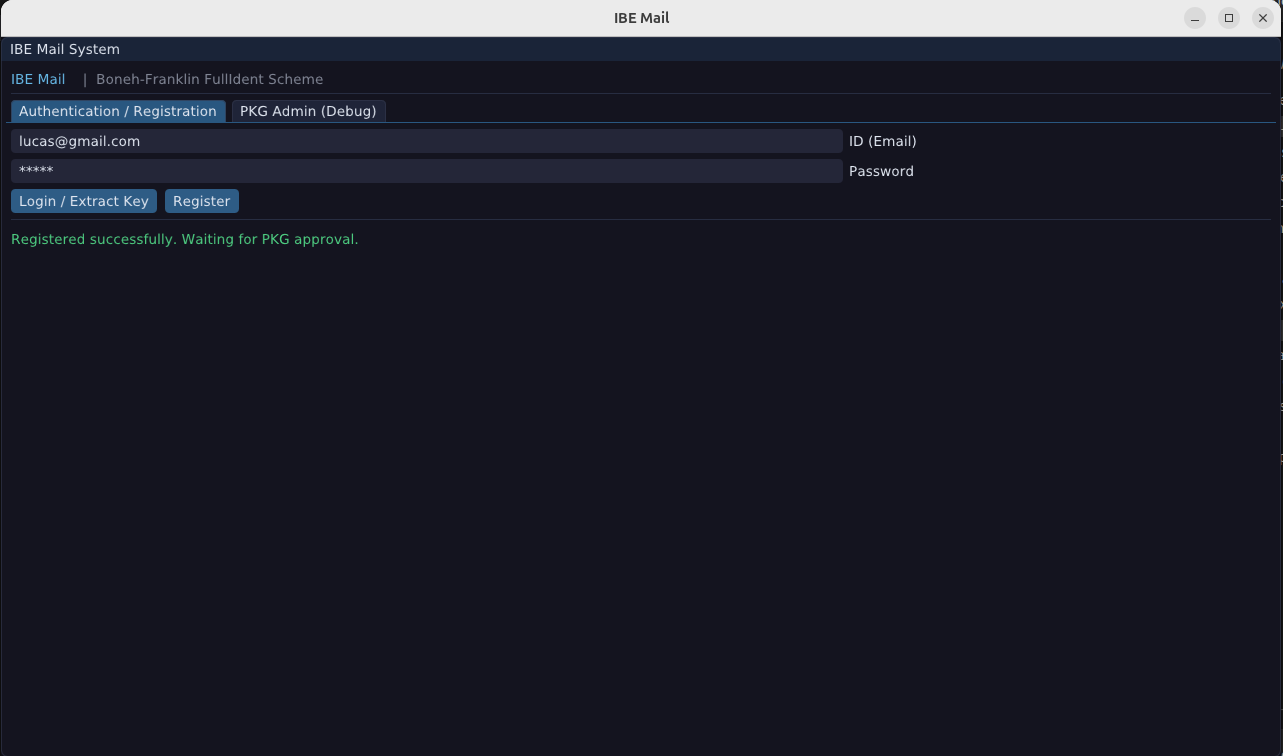
\includegraphics[width=0.9\textwidth]{images/2_pkg_pending.png}
    \caption{Solicitações pendentes.}
    \label{fig:pkg_pending}
\end{figure}

\begin{figure}[htb]
    \centering
    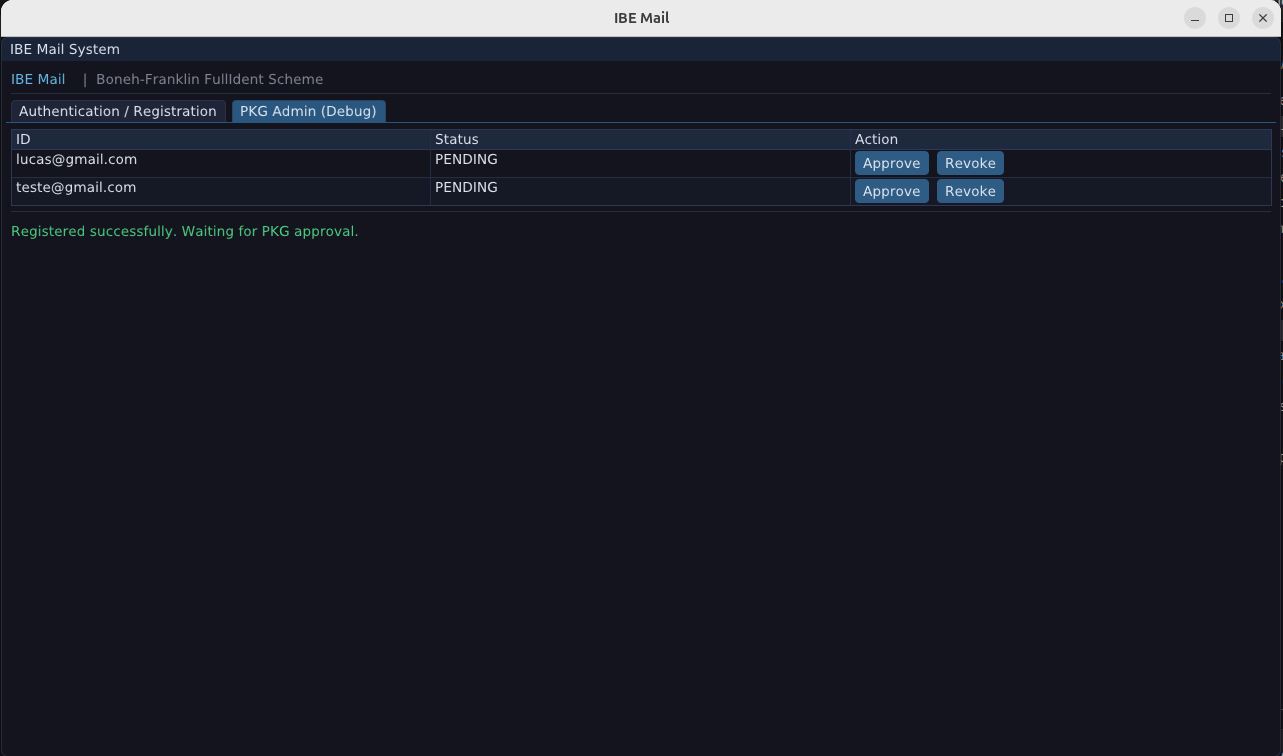
\includegraphics[width=0.9\textwidth]{images/3_pkg_approved.png}
    \caption{Aprovação de usuários.}
    \label{fig:pkg_approved}
\end{figure}

Com a aprovação, o usuário pode fazer o \textit{login} normalmente (Figura \ref{fig:auth_success}), obtendo acesso instantâneo ao uso de sua chave privada para a decifragem de mensagens.

\begin{figure}[htb]
    \centering
    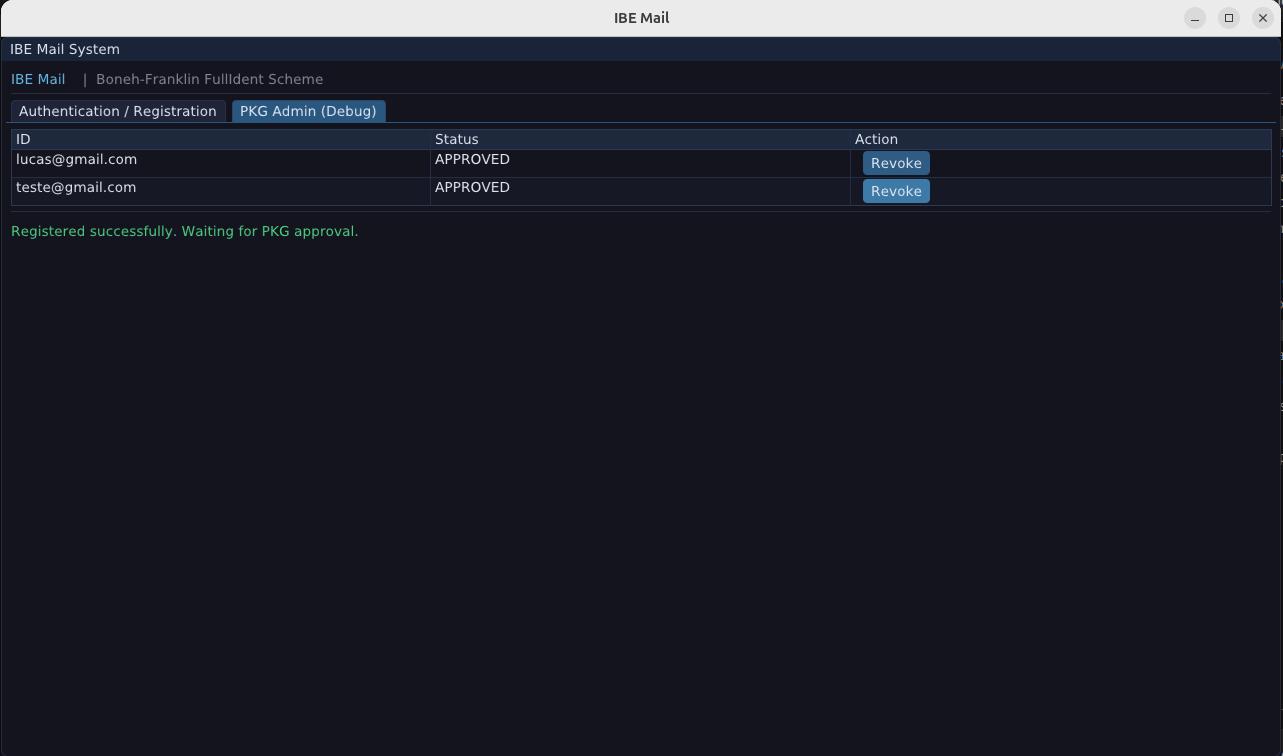
\includegraphics[width=0.9\textwidth]{images/4_auth_success.png}
    \caption{Usuário autenticado com sucesso e pronto para operar.}
    \label{fig:auth_success}
\end{figure}

\section{Troca de Mensagens}

Com usuários registrados no sistema, é possível demonstrar o roteamento e a decifragem de mensagens. A Figura \ref{fig:compose} mostra a formulação de um novo e-mail cifrado enviado de uma identidade para outra.

\begin{figure}[htb]
    \centering
    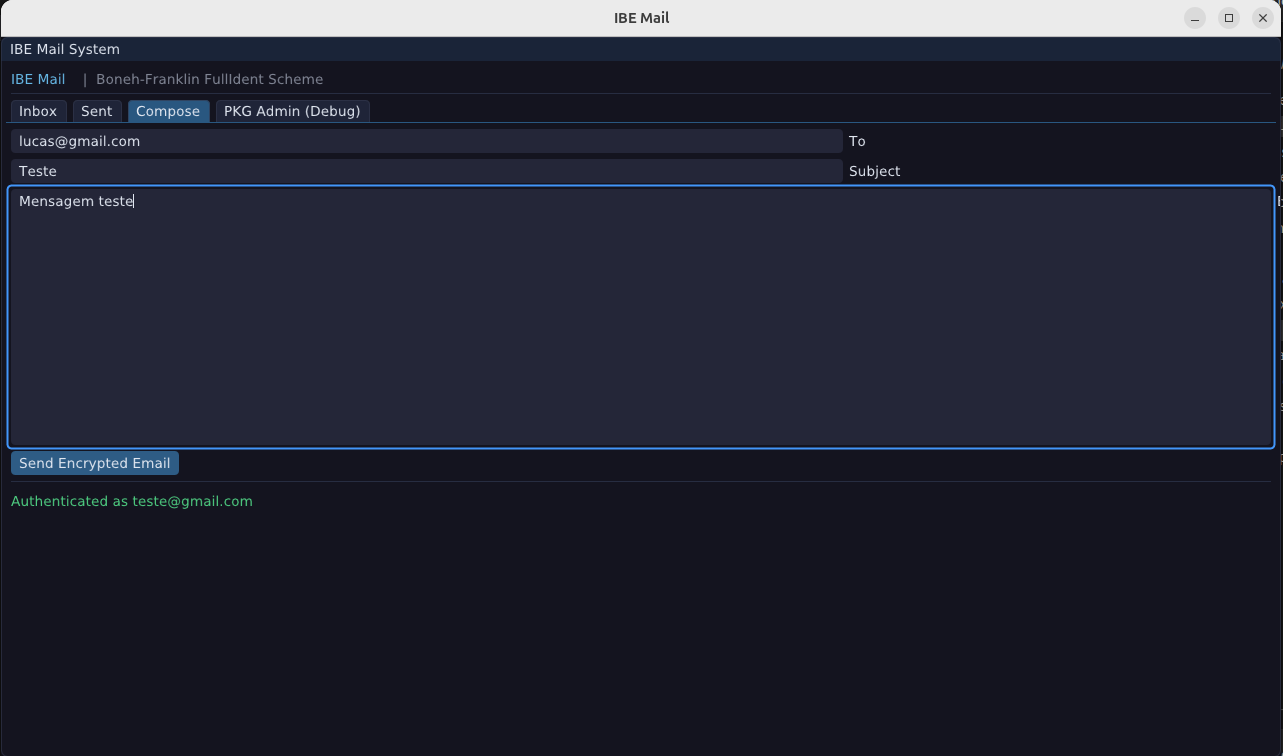
\includegraphics[width=0.9\textwidth]{images/5_compose.png}
    \caption{Interface de envio de mensagens cifradas.}
    \label{fig:compose}
\end{figure}

O remetente, após enviar o texto, pode observar na aba \textit{Sent} (Figura \ref{fig:sent}) os e-mails emitidos. O programa exibe o conteúdo do arquivo físico \texttt{.ibemail} gerado. É importante notar que o rementente não pode ler a mensagem que ele mesmo enviou, dado que o texto foi cifrado para a chave pública do destinatário.

\begin{figure}[htb]
    \centering
    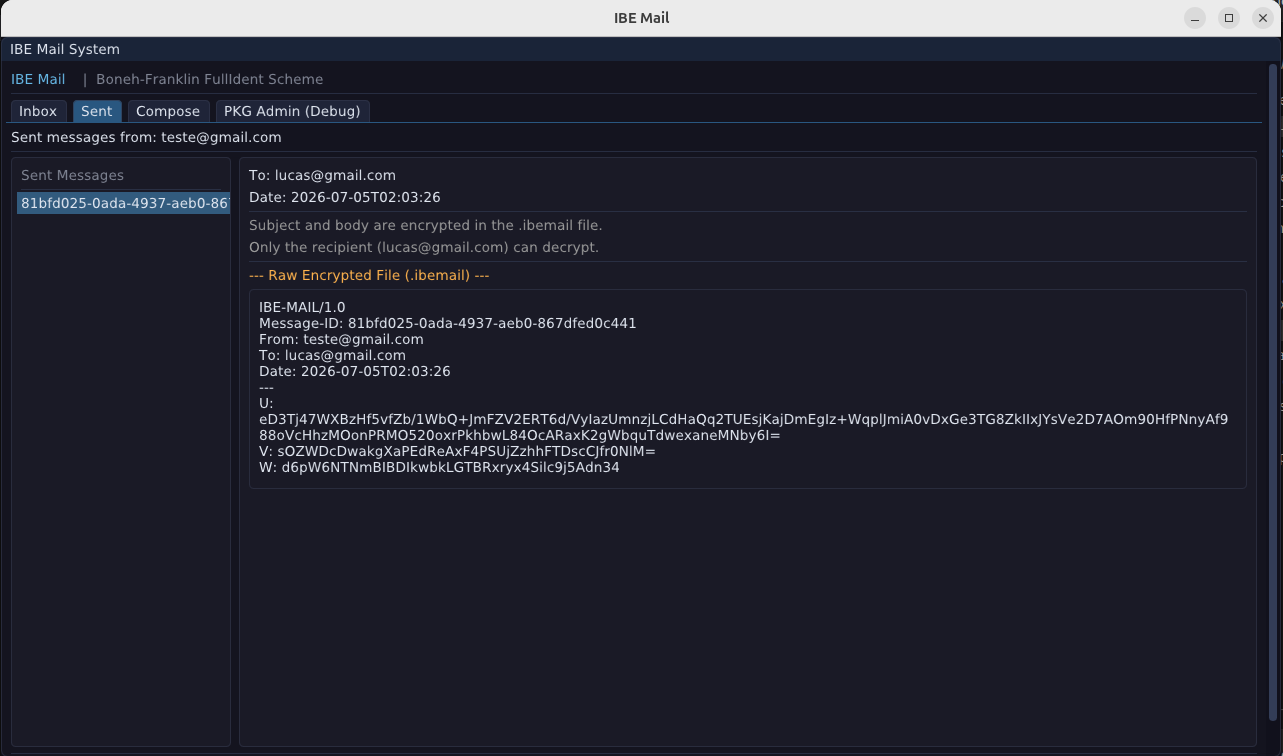
\includegraphics[width=0.9\textwidth]{images/6_sent.png}
    \caption{Aba de enviados exibindo os blocos de texto cifrado em Base64.}
    \label{fig:sent}
\end{figure}

Ao abrir a caixa de entrada (\textit{Inbox}) do destinatário \texttt{lucas@gmail.com}, o algoritmo \textit{Decrypt} extrai e reverte os blocos de informação utilizando a chave privada gerada na primeira etapa. A mensagem é decifrada de forma legível e perfeitamente íntegra (Figura \ref{fig:inbox}).

\begin{figure}[htb]
    \centering
    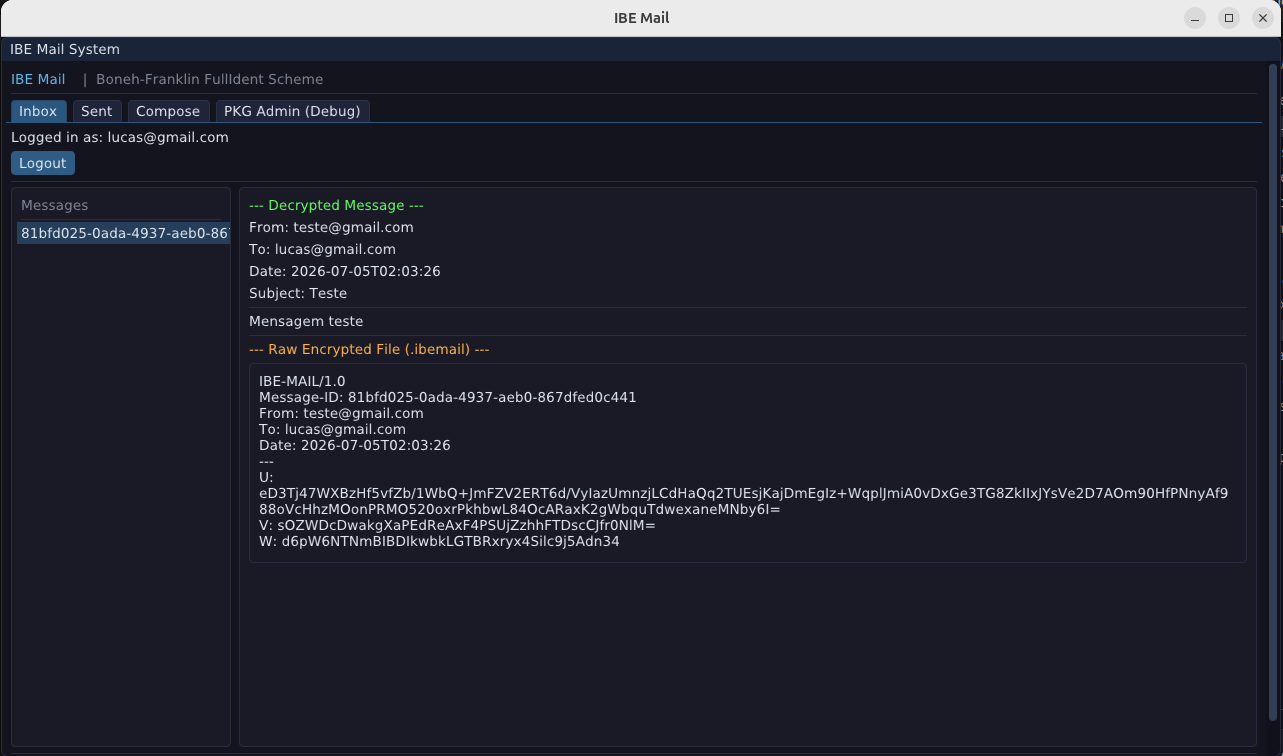
\includegraphics[width=0.9\textwidth]{images/7_inbox.png}
    \caption{Mensagem decifrada e lida com sucesso pelo destinatário.}
    \label{fig:inbox}
\end{figure}

\section{Segurança IND-ID-CCA2}

A implementação utiliza a transformação de Fujisaki-Okamoto (FO) para garantir que mensagens alteradas sejam ativamente rejeitadas no momento da decifragem, inviabilizando ataques de falsificação de texto cifrado.

Para provar esta propriedade na prática, o arquivo original de uma mensagem foi deliberadamente alterado via editor de código (Figura \ref{fig:file_alteration}), modificando-se um caractere do cifrotexto (bloco $U$).

\begin{figure}[htb]
    \centering
    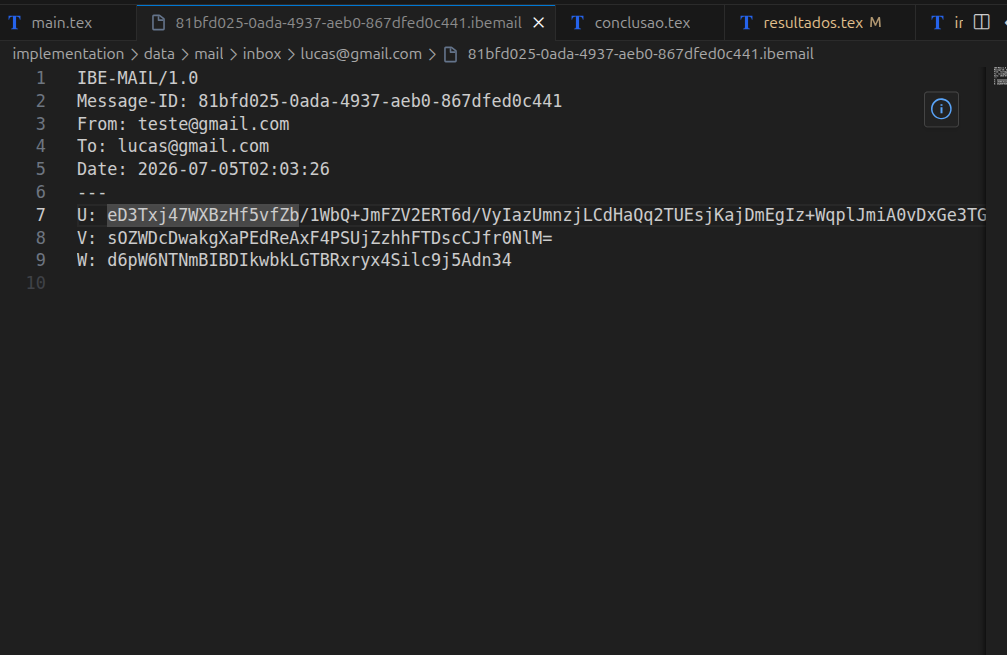
\includegraphics[width=0.9\textwidth]{images/8_file_alteration.png}
    \caption{Alteração maliciosa injetada no arquivo \texttt{.ibemail} utilizando um editor.}
    \label{fig:file_alteration}
\end{figure}

Ao retornar para a interface do programa e tentar ler a mensagem adulterada, a verificação de consistência hash de Fujisaki-Okamoto ($U = r \cdot P$) falha. O sistema detecta a violação, lança um erro e impede a leitura (Figura \ref{fig:cca2_rejection}), garantindo a resiliência (CCA2) do protocolo IBE contra adulterações ativas.

\begin{figure}[htb]
    \centering
    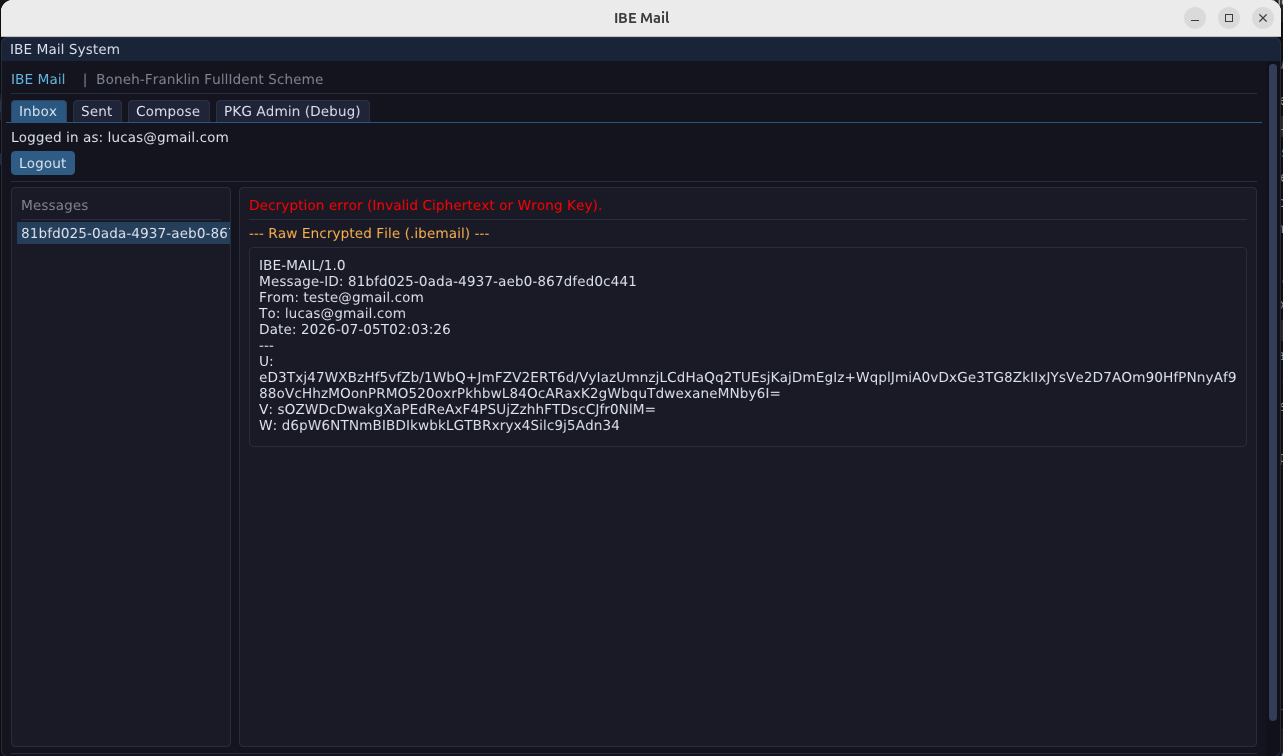
\includegraphics[width=0.9\textwidth]{images/9_cca2_rejection.png}
    \caption{Rejeição imediata do cifrotexto devido a quebra de integridade (CCA2).}
    \label{fig:cca2_rejection}
\end{figure}

\section{Identidades Temporais (Cifragem para o Futuro)}

Uma das características mais marcantes da Criptografia Baseada em Identidade é a capacidade de cifrar dados sigilosos para chaves que sequer foram geradas pelo PKG.

No teste final, uma mensagem foi endereçada à identidade \texttt{teste2@gmail.com|2026-06} (Figura \ref{fig:time_sent}), demonstrando o particionamento de uma identidade no tempo (útil para processos de revogação periódica natural). O e-mail foi cifrado utilizando essa estrutura (\textit{string}) literal como chave pública matemática, sem que a chave privada real existisse naquele momento.

\begin{figure}[htb]
    \centering
    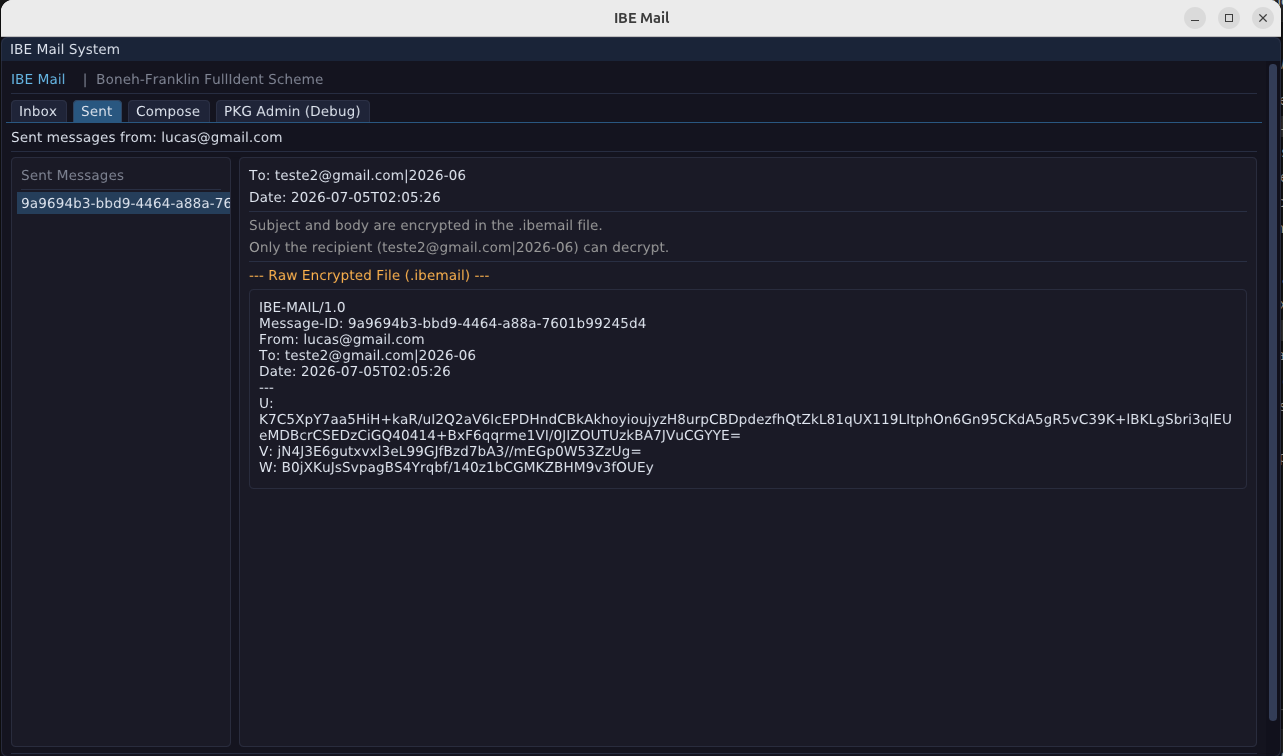
\includegraphics[width=0.9\textwidth]{images/10_time_sent.png}
    \caption{Envio de e-mail assíncrono para uma identidade contendo partição de data.}
    \label{fig:time_sent}
\end{figure}

Posteriormente, a identidade exata particionada (\texttt{teste2@gmail.com|2026-06}) foi registrada no sistema e aprovada no PKG. Ao logar com essa credencial temporal, o usuário conseguiu recuperar sua chave privada retroativamente e ler as mensagens que lhe foram destinadas, comprovando na prática o dinamismo e o roteamento exato da abordagem de Boneh-Franklin (Figura \ref{fig:time_inbox}).

\begin{figure}[htb]
    \centering
    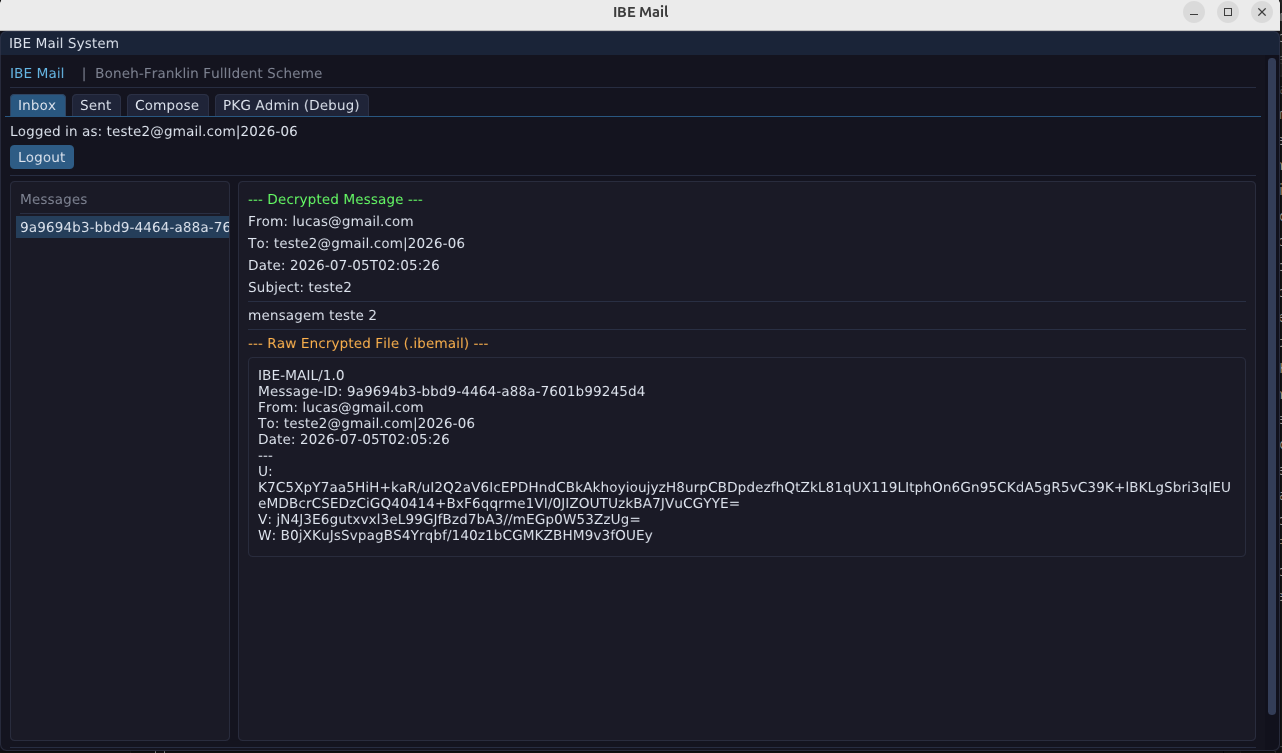
\includegraphics[width=0.9\textwidth]{images/11_time_inbox.png}
    \caption{Usuário logado sob a identidade de tempo específica para recuperar as mensagens.}
    \label{fig:time_inbox}
\end{figure}
